\begin{figure}[htpb]
	\centering\capstart{}
	\subfloat[\(\Re\big\{\pixel{\mathcal{EG}}\big\}\)]  % chktex 21
	{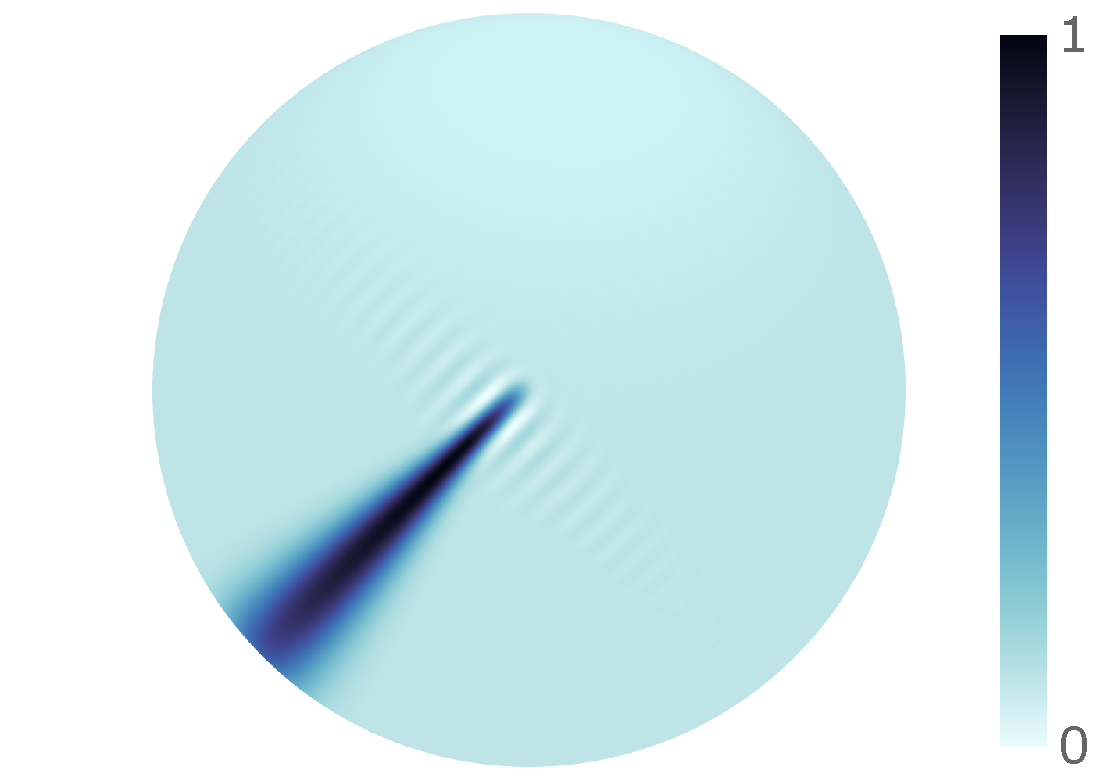
\includegraphics[trim={4 7 3 6},clip,width=.5\textwidth]{elongated_gaussian_1tsig_1psig10_L128_res512_real_norm.pdf}}
	\hfill
	\subfloat[\(\Re\big\{\pixel{(\translation{\omega'}\mathcal{EG})}\big\}\)]  % chktex 21
	{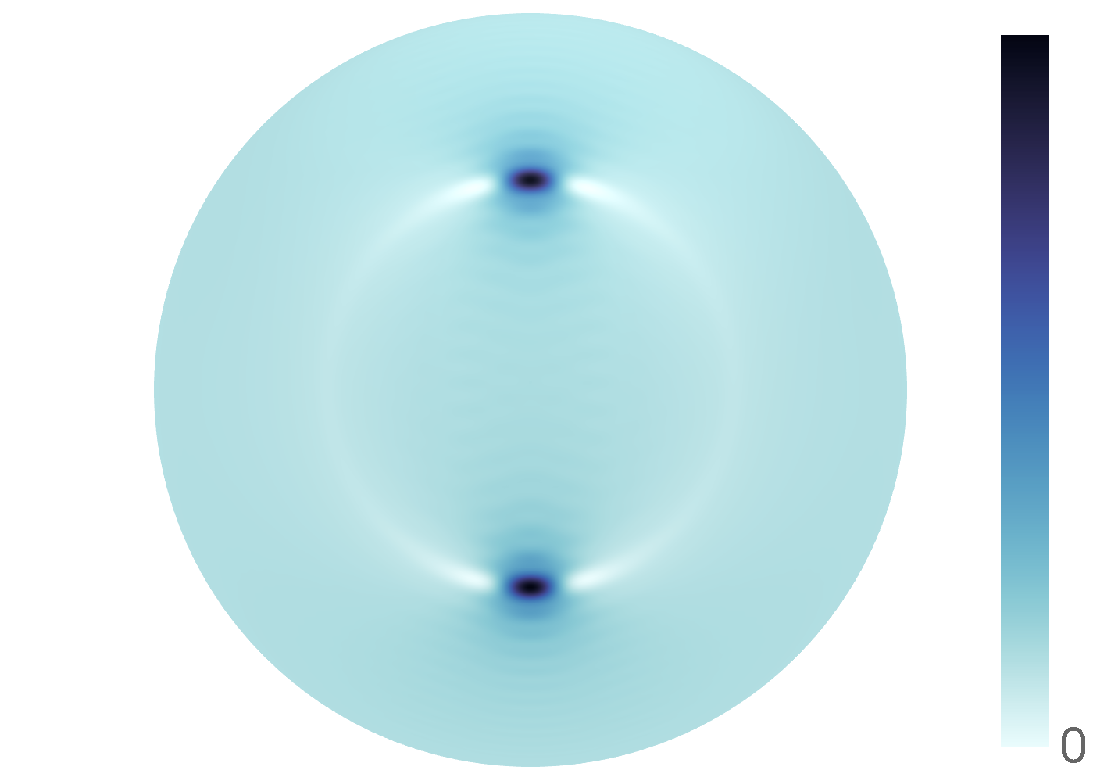
\includegraphics[trim={4 7 3 6},clip,width=.5\textwidth]{elongated_gaussian_1tsig_1psig10_L128_translate_alpha3pi4_beta1pi8_res512_real_norm.pdf}}
	\caption[
	An elongated Gaussian on the north pole and then translated
	]{
	Presented in panel (a) is an elongated Gaussian with parameters \((\mean{\theta},\mean{\phi},\sigma_{\theta},\sigma_{\phi}) = (0,\pi,10^{0},10^{-1})\) on the north pole (bandlimited at \(L=128\)), \cf{} \cref{eq:chapter3_elongated_gaussian} --- where the central bar in the plot extends over half of the sphere.
	The elongated Gaussian is then translated to some \(\omega'=(\theta',\phi')\), as shown in panel (b).
	The even azimuthal symmetry in the initial kernel definition results in the two localised components at \(\phi'\) and \(-\phi'\) under translation.
	The colour is between zero and one, reflecting the scaled intensity of the field.
	}\label{fig:chapter3_elongated_gaussian}
\end{figure}
